\documentclass[border=4pt]{standalone}
\usepackage{tikz}
\usetikzlibrary{arrows.meta}
\begin{document}
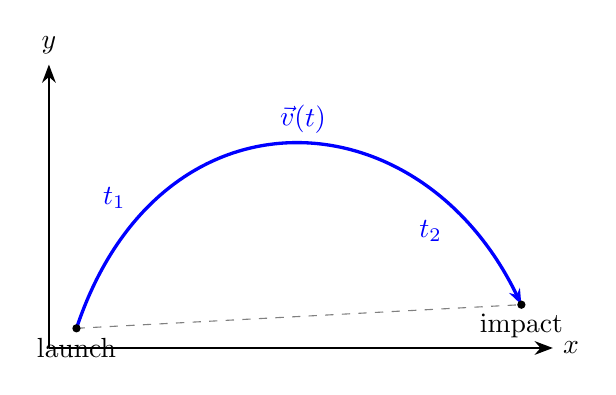
\begin{tikzpicture}[auto,>=Stealth]
  \draw[->,thick] (0,0) -- (6.4,0) node[right] {$x$};
  \draw[->,thick] (0,0) -- (0,3.6) node[above] {$y$};
  \draw[blue,very thick,-{Stealth[length=2mm]}]
    (0.35,0.25) .. controls (1.4,3.4) and (4.7,3.25) .. (6.0,0.55)
    node[pos=.18] {$t_1$}
    node[pos=.52,sloped,above] {$\vec v(t)$}
    node[pos=.82,swap] {$t_2$};
  \draw[dashed,gray] (0.35,0.25) -- (6.0,0.55);
  \fill (0.35,0.25) circle (1.5pt) node[below] {launch};
  \fill (6.0,0.55) circle (1.5pt) node[below] {impact};
\end{tikzpicture}
\end{document}
